% Sample file for AES paper
\documentclass{aes2e}
\usepackage{amsmath}
\usepackage{float}
\usepackage{microtype} % Better typography
\usepackage{xcolor}    % Color support
\DeclareMathOperator*{\argmax}{arg\,max}

\renewcommand{\printbiography}{}

%FIX SIDENUMBBER START
\makeatletter
\def\ps@plain{%
  \let\@mkboth\@gobbletwo
  \def\@oddhead{}%
  \def\@evenhead{}%
  \def\@oddfoot{\hfil\thepage\hfil}%
  \def\@evenfoot{\hfil\thepage\hfil}%
}
\makeatother
\pagestyle{plain}
%FIX SIDENUMBBER SLUT

% Metadata Information
\jyear{2025}
\jmonth{December}


\begin{document}

% Page heads
\markboth{Villadsen et al.}{I.C.U.M: IMU-Controlled UltraWideband Mesh}

% Title portion
% Added some color and a rule
\title{I.C.U.M - IMU Controlled Ultra-wideband Mesh System \\[\baselineskip] \color{black!80}\hrule height 0.5pt}

%Author Info.
\authorgroup{
\vspace{5pt}
\textsc{Authors} \\
\vspace{5pt}
\author{Benjamin M. Villadsen, \quad Benjamin S. Larsen, \quad Muad Ghanim,} \\
\author{Thor C. Koustrup-Müller, \quad Daniel Brenet}
\email{bmvi21, bsla21, muad, tkoust21, dbrene21 @student.aau.dk}
\vspace{15pt}
\textsc{Supervisor} \\
\vspace{5pt}
\author{
Tung "Gamer" Kieu
}
\email{tungkvt@cs.aau.dk}
\affil{Aalborg University, Copenhagen S, Denmark}
\affil{21. December 2025}
}

%Abstract
%Purpose: A short summary of the entire study—what you did, how, and why it matters.
%Typical length: 150–250 words
%Should include:
%Background/problem: Why the study was needed
%Objective: What the paper aims to achieve
%Methods: Brief overview of techniques or datasets used
%Results: Main findings or performance metrics
%Conclusion: Key takeaway or implications
\abstract{
\noindent \textbf{Abstract} --- This paper presents the IMU-Controlled UltraWideband Mesh (I.C.U.M), a decentralized localization framework designed to enable autonomous swarm compliance in GPS-denied environments without reliance on static anchors. By fusing peer-to-peer Ultra-Wideband (UWB) ranging with low-cost Inertial Measurement Units (IMUs), we propose a distributed spring-relaxation algorithm that allows mobile agents to maintain a rigid relative coordinate frame solely through local interactions. To address the critical energy constraints of battery-powered swarms, we introduce an Event-Triggered Messaging (ETM) protocol that gates radio transmissions based on inertial motion detection. Empirical validation through the open-source I.C.U.M-SIM environment demonstrates that this architecture reduces network communication overhead by 76.17\% compared to periodic baselines while maintaining sub-meter formation accuracy (RMSE $\approx$ 0.1m). Furthermore, we identify a "Rigidity Transition" in network scalability, showing that node density acts as a catalyst for geometric convergence. The proposed system offers a robust, energy-efficient foundation for rapid-deployment search-and-rescue teams and subterranean robotics.}


\vspace{10pt}
\noindent\textbf{Keywords:} Cooperative Localization, Ultra-Wideband (UWB), Inertial Measurement Unit (IMU), Event-Triggered Messaging, Wireless Sensor Networks.}


\maketitle

%Head 1
%\section{INTRODUCTION}
%Head 1
%\section{INTRODUCTION}


\thispagestyle{plain}

\section{INTRODUCTION}

\begin{figure*}[t!]
    \centering
    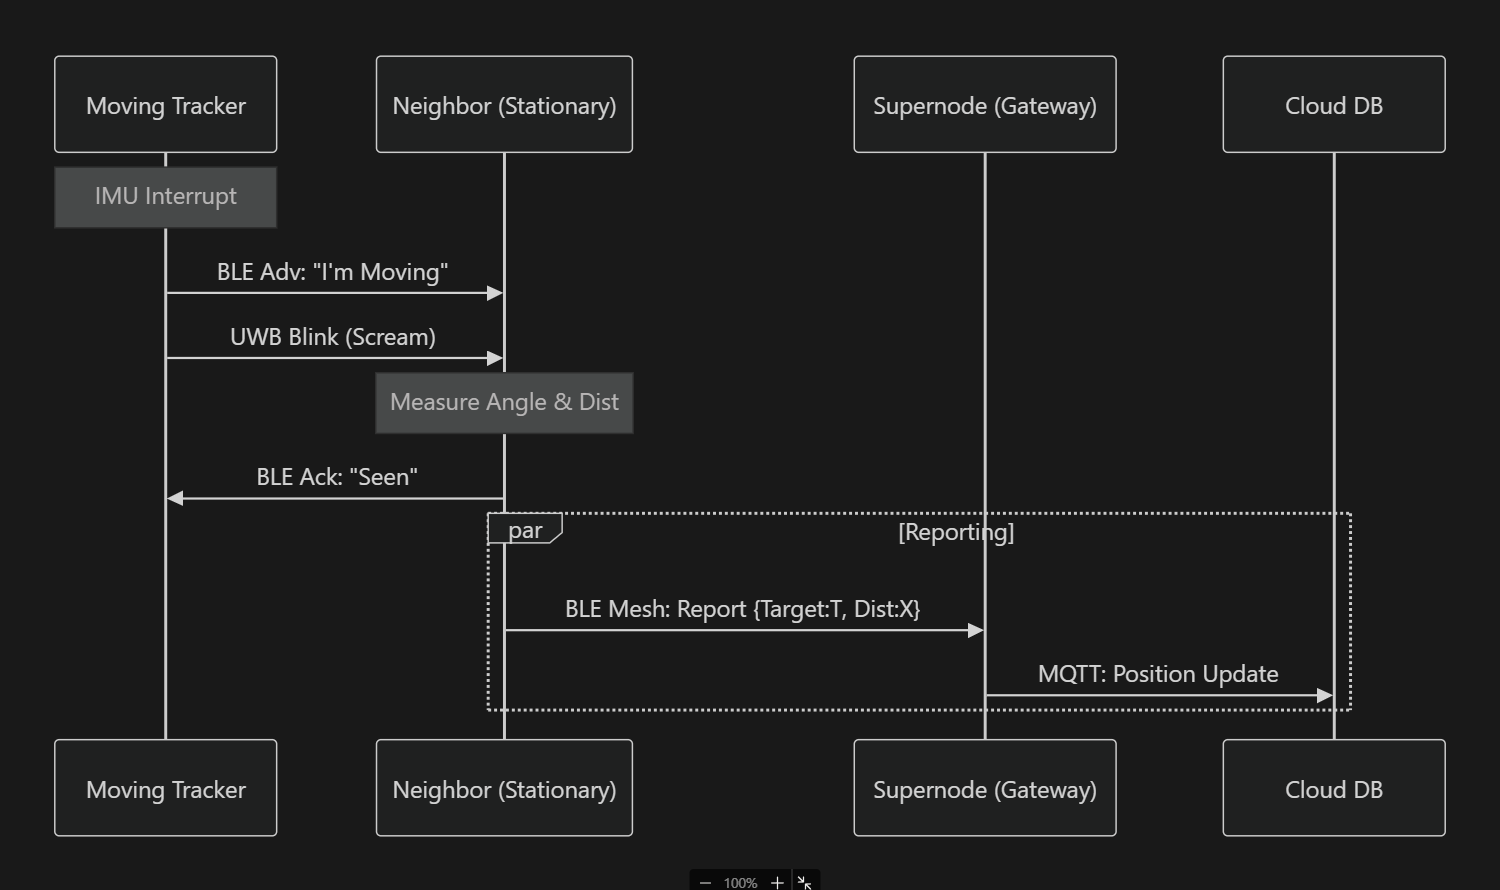
\includegraphics[width=0.9\textwidth]{images'nshi/comm.png}
    \caption{\textbf{System Overview.} The I.C.U.M. ecosystem integrates a realistic discrete-event simulator (ICUM-SIM) with a novel distributed firmware architecture. Nodes leverage event-triggered messaging (ETM) driven by inertial dynamics to maintain a rigid formation without static infrastructure, balancing localization accuracy with long-term energy efficiency.}
    \label{fig:system_overview}
\end{figure*}
%Purpose: Show how your work fits into the existing research landscape.
%Should include:
%Summaries of similar studies or technologies
%Comparisons of their strengths, limitations, or approaches
%Justification for why your method is new or necessary
\noindent Cooperative localization \cite{locatingthenodes} \cite{cooporativelocalizationinwirelessnetworks} \cite{localizationcooperative} is a localization method that uses wireless sensor nodes to leverage system architecture and network topology to estimate the positioning of these nodes. Through estimation of positions relative to each other, the nodes in the network can, with a high degree of accuracy, find the positioning of any entity within the system network. The positioning data can be either relative to each other without providing any concrete location, or, through the use of an anchor in the system architecture and topology, or coordinates computed based on the anchor coordinates and subsequent node measurements. Additionally, cooperative localization systems, being inherently distributed systems, are classified as either being centralized or decentralized \cite{wirelesssensornetworklocalizationtechniques}. The most significant differences in operational effectiveness are the tradeoffs in scalability, efficiency, and accuracy. Centralized networks are more difficult to scale properly, while decentralized networks can be less accurate and take longer to converge to a location solution.

\noindent There are mainly two techniques used to compute the distance between two nodes \cite{wirelesssensornetworklocalizationtechniques}, namely Received Signal Strength Indication (RSSI) \cite{CollaborativeLocalizationWithReceivedSignalStrengthinWirelesSensorNetworks} and Time of Flight (ToF) \cite{RadioFrequencyTimeofFlightDistanceMeasurementforLowCostWirelessSensorLocalization}. By measuring the energy exerted by a device, the strength of a radio signal can be estimated in milliwatts. Still, due to the nature of these signals, measurements become extremely small and difficult to work with. To work with these signals more easily, they are instead measured in decibel milliwatts (dBm). This non-SI logarithmic unit is measured negatively, with numbers closer to 0 indicating a stronger signal. This approach leverages any lack of synchronization between the nodes and the ubiquitous nature of technologies like Wi-Fi and Bluetooth Low Energy (BLE), which can easily measure RSS, making it great for pre-existing networks. However, RSS is extremely volatile, as a few obstacles in a non-static environment can severely impact the measured values.\\

\noindent Alternatively, UWB sensors, which are more accurate but require more power, can take advantage of ToF natively \cite{OnperformancestudyofUWBrealtimelocatingsystem}. Signals can be exchanged between two time-synchronized nodes to estimate the distance between them by comparing the time when the signal was sent by the first node and received by the second. Since radio waves travel at the speed of light, even a small difference in their clocks can lead to significant estimation errors, which means that additional computational power must be spent to ensure that all nodes are time-synchronized, a task that becomes increasingly difficult in large networks. To remedy this, UWB offers support for Two-Way Ranging (TWR), which works as stated above, but with an added message sent from the second node back to the first to calculate potential time differences \cite{Real-TimeAnchorNodeSelectionforTwo-Way-Ranging(TWR)Ultra-Wideband(UWB)IndoorPositioningSystems}.\\

\noindent Both RSS and TWR-ToF require a way to tell in which direction the measured distance is, which is done by calculating the Angle of Arrival (AoA) \cite{AnguLoc}. It’s important to note that a single UWB sensor cannot measure the AoA. It is determined by comparing the phase of the received signal across two or more antennas placed on the same UWB device, allowing the direction of the incoming signal to be estimated. Consequently, UWB nodes employing TWR-ToF were selected as the sensing technology for the cooperative localization system proposed in this paper.\\

%Cooperative localization refers to the process in which multiple agents (e.g., robots, vehicles, or sensors) estimate their positions by sharing observations and relative measurements. 
\noindent The primary advantage of cooperative localization is improved accuracy. By combining independent sensor data, agents reduce individual uncertainty and mitigate drift inherent to inertial and dead-reckoning methods \cite{CooperativeLocalizationApproachforMulti-RobotSystemsBasedonStateEstimationErrorCompensation}. Cooperative localization also enhances robustness in environments where GPS or local sensing is unreliable, since agents can provide corrective information to one another \cite{CooperativeLocalizationUsingDistanceMeasurementsforMobileNodes}. Furthermore, the approach increases fault tolerance—individual sensor failures have less impact—and supports scalability in multi-agent systems by distributing sensing responsibilities across the network \cite{Fault-TolerantMulti-ModalLocalizationofMulti-RobotsonMatrixLieGroups}. Battery performance is also a vital aspect of distributed networks if the nodes are deployed without a constant source of power. One aspect of distributed cooperative localization systems that can largely affect battery performance is the communication between nodes. Nodes that attempt to update location information despite no significant real-world change will waste a significant amount of energy \cite{EnergyEfficiencyOptimizationofCooperativeCommunicationinWirelessSensorNetworks}, while not updating location information often enough will impair the systems performance \cite{Space-TimeHierarchicalGraphBasedCooperativeLocalizationinWirelessSensorNetworks}. These two factors highlight the balance between sufficient and efficient communication needed for cooperative localization systems, which is what our research aims to achieve. Our system combines inertial movement readings to effectively detect when a location update is required. By only initiating location updating when needed, the nodes will not send superfluous location updates, and only initiate communication when needed.

\subsection*{Contributions}
\noindent This paper makes the following contributions to the field of infrastructure-free cooperative localization:
\begin{enumerate}
    \item \textbf{Event-Triggered Architecture:} We propose an IMU-gated communication protocol that reduces network overhead by over 75\% while maintaining sub-meter relative accuracy, effectively balancing energy efficiency with formation integrity.
    \item \textbf{Anchor-Free Formation Rigidity:} We demonstrate that a decentralized "spring-mass" optimization can converge to a rigid geometric formation (RMSE $< 0.1m$) solely from peer-to-peer UWB ranging, eliminating the need for expensive static infrastructure or GPS availability.
    \item \textbf{Battery-Aware Topology Control:} We introduce a hierarchical leader election algorithm that dynamically rotates cluster leadership based on energy reserves and connectivity.  Simulation results confirm this mechanism prevents the "death spiral" of critical nodes and extends the functional lifetime of the network.
    \item \textbf{Open Source Simulation Framework:} We provide ICUM-SIM, a verified component-based simulator for prototyping distributed localization algorithms with realistic physics, hardware emulation, and energy depletion models.
\end{enumerate}









\section{Related Work}
%https://www.researchgate.net/publication/378119265_Ad_Hoc_Mesh_Network_Localization_Using_Ultra-Wideband_for_Mobile_Robotics
\noindent Localization in GPS-denied environments commonly leverages UWB sensing due to its robustness to multipath and centimeter-level accuracy. Prior systems typically rely on static anchors or assume robots remain stationary during initialization. As summarized by Juston et al.
\cite{AdHocMeshNetworkLocalizationUsinUltra-WidebandForMobileRobotics}, most UWB localization methods either (1) use regression-based multilateration followed by Kalman filtering or (2) apply Monte Carlo-style sampling approaches. Although improved non-linear least-squares techniques and multi-tag configurations increase robustness, these frameworks still constrain network topology by requiring fixed reference nodes or stable visibility conditions.\\

\noindent Filtering methods such as the Extended or Unfiltered Kalman Filter are widely used to refine UWB-based estimates, yet they remain sensitive to NLOS noise and often depend on supplemental sensors. Approaches incorporating mobile beacons exist, but they generally assume the beacons themselves remain globally localized or static relative to the agent.\\

\noindent The work of Juston et al. \cite{AdHocMeshNetworkLocalizationUsinUltra-WidebandForMobileRobotics} advance the field by allowing all nodes, including anchors, to be mobile, enabling a decentralized ad-hoc mesh in which localization propagates dynamically. This shift away from reliance on static infrastructure aligns with our research goal of developing resilient localization methods suitable for highly dynamic multi-robot environments.\\
%hej daniel
%bridge de her to afsnit mayb?

\noindent Han et al. \cite{ANovelCooperativeLocalizationMethodBasedonIMUandUWB} 
Prior work on cooperative localization largely relies on wireless ranging technologies such as Bluetooth, Wi-Fi, ZigBee, and UWB, typically requiring at least three auxiliary nodes to triangulate position using AOA, TOA, or TDOA methods. These approaches depend solely on anchor measurements and overlook motion information from the target node, leading to limited robustness and high infrastructure cost in dynamic environments 
To address these limitations, hybrid sensor-fusion methods combining inertial sensing with wireless ranging have been explored, demonstrating improved accuracy and drift compensation in GPS-denied or cluttered environments. Han et al. propose an IMU/UWB cooperative localization method that reduces the required auxiliary nodes to one by integrating DR and UWB measurements via an Adaptive Ant Colony Optimization Particle Filter (AACOPF), enabling accurate estimation of both position and azimuth even without prior initialization.\\ 


%How do we propose a use for IMU, short and informal
\noindent Building on these related works, our research draws directly from the demonstrated strengths of UWB-based cooperative localization systems, particularly their robustness in GPS-denied environments and their ability to fuse heterogeneous sensor inputs for improved accuracy. Prior studies highlight both the promise and limitations of multilateration, regression-based estimation, and Kalman-filter refinements \cite{AdHocMeshNetworkLocalizationUsinUltra-WidebandForMobileRobotics}, as well as the benefits of integrating inertial sensing to compensate for drift and reduce reliance on dense anchor deployments \cite{ANovelCooperativeLocalizationMethodBasedonIMUandUWB}.Ultimately, the reviewed literature provides the methodological foundation and justification for developing a resilient, decentralized localization framework suited for the dynamic environments our system targets. 


%\subsection*{3.3.2 Angle og Arrival (AoA) Constraint}
%\noindent The simulator incorporates Angle of Arrival (AoA) data to constrain the rotational freedom of the graph. If node $i$ measures node $j$ at angle $\phi_{ij}$ relative to its own heading $\theta_i$, the angular error is:
%\begin{equation}
   %e_{angle} = wrap(\theta_i + \theta_{ij} - atan2(y_j - y_i, x_j-x_i))
%\end{equation}

\section{Algorithms \& System Model}
\noindent Unlike traditional centralized localization systems that rely on raw trilateration, this project's proposed solution, namely "ICUM" system, implements a distributed state machine where node roles are dynamic and position estimation is performed via a cooperative graph optimization algorithm.

\subsection{Dynamic Role Management}
\noindent The network operates as a Destination-Oriented Directed Acyclic Graph (DODAG) for sending messages. Nodes autonomously switch between roles based on their connectivity state and sensor readings. Let $R_i(t)$ denote the role of the node $i$ at time $t$. The state space is defined as: 
\begin{equation}
    R \in \{ROOT, LEADER, RELAY, IDLE, ISOLATED\}
\end{equation}
A node in the state $IDLE$ must send its messages "up" to either $RELAY$s or $LEADER$s, hence why the messaging strategy is based on DODAG. Transitions are governed by the tuple ($H_{gw}, N{neighbors},T_{iso}$), where $H_{gw}$ is the hop count to a gateway, $N_{neighbors} = 0$ for a duration $t > T_{iso}$. A node promotes itself to $R = LEADER$ if it wins the local election process defined in section 3.4.

\subsection{Hardware}
\noindent Since every node needs the capabilities to fill whatever role the system requires at any given state, the hardware stack must be homogeneous. Below is a tentative hardware specification that fulfils all the requirements of the system:
\begin{itemize}
    \item \textbf{Computation}: MCU (e.g., Nordic nRF52/53 or STM32)
    \item \textbf{Sensors}: 6-axis IMU (Accelerometer/Gyro)
    \item \textbf{Communication}: BLE for Mesh data \& Signalling
    \item \textbf{Ranging}: UWB (DW3000) for TWR Distance \& AoA
    \item \textbf{Backhaul}: LTE-M / NB-IoT
\end{itemize}
MCUs are ideal for distributed systems \cite{MicrocontrollerUnit-BasedWirelessSensorNetworkNodes:AReview}, given their low latency, ultra-low power consumption, and durability in systems that never shut down. As for the inertial movement detector, any low-power accelerometer can be used, but IMU sensors have been chosen for their accuracy and potential for self-optimization based on inertial movement. The communication strategy will revolve around many instances of one-to-one communication, making BLE an effective option for sending and receiving messages. Note that over large distances, BLE can experience significantly reduced effectiveness, so this choice may need reconsidering depending on the application domain. As mentioned before, UWB will be used for ranging, and if a node is unable to detect any $LEADERS$ or $RELAYS$, it will use LTE-M, which is effective in low-power areas, to detect its own location with GPS as well as possible. Naturally, this goes against the design philosophy and intended application of the system, but it is only used as a backup option for when no other location detection or computation is available.

\subsection{States and Communication}
\noindent The states related to the movement of the wireless sensor nodes are depicted below in figure \ref{fig:states}. When a node joins the network, the initial internal state is $STATIONARY$, even if the node itself is physically moving. When its inertial sensor is turned on, it will start to monitor its movement, and if it exceeds $0.5G$, it will transition to the $MOVING$ state. While moving, it will turn off its relay properties, preventing it from forwarding messages from neighbouring nodes to $LEADERS$. Moving nodes are naturally volatile, making their relay capabilities more unreliable and unstable, which is the basis for this design choice. While moving, nodes will repeatedly perform UWB blinking to receive location information from the neighbouring nodes. A neighbouring node that responds to UWB ranging must send an acknowledgment to ensure that the UWB blinking was noticed by at least one neighbouring node. If a $MOVING$ node has not received acknowledgements for 30 seconds, or a $STATIONARY$ node has not detected UWB blinking for 30 seconds, it will transition to the $ISOLATED$ state. In this state, the node will continuously scan for nearby mesh networks in an attempt to join a cluster, and without the possibility for cooperative localization, it will fall back to GPS despite potentially being in a GPS-denied environment. The location will be transmitted to the cloud regardless of accuracy, and if a mesh network is found, depending on the movement of the node, it will either transition back to $STATIONARY$ or $MOVING$.\\

\noindent Illustrated in figure \ref{fig:sequence} is a sequence diagram modelling the communication between the different nodes and cloud service. The $Moving\  Tracker$ object will initiate communication by sending a message to any $Neighbouring\ Nodes$ to which they will respond by measure the AoA and euclidean distance from themselves to the messaging node. They will follow up with an acknowledgment and the location information that the $Moving\ Tracker$ will use to update its internal location. This will then be sent to the nearest $Leader$ node, and forwarded to the $Cloud$. if the $Moving\ Tracker$ is in the $ISOLATED$ state, it will send its own GPS location directly to the $Cloud$, however inaccurate it may be. 

\begin{figure*}[t] %float with two figures
\centering
\includegraphics[width= 1\linewidth]{images'nshi/stateDiagram.png}
\caption{State diagram of the wireless sensor nodes depicting the relation between states and transitions\label{fig:states}}\bigskip 
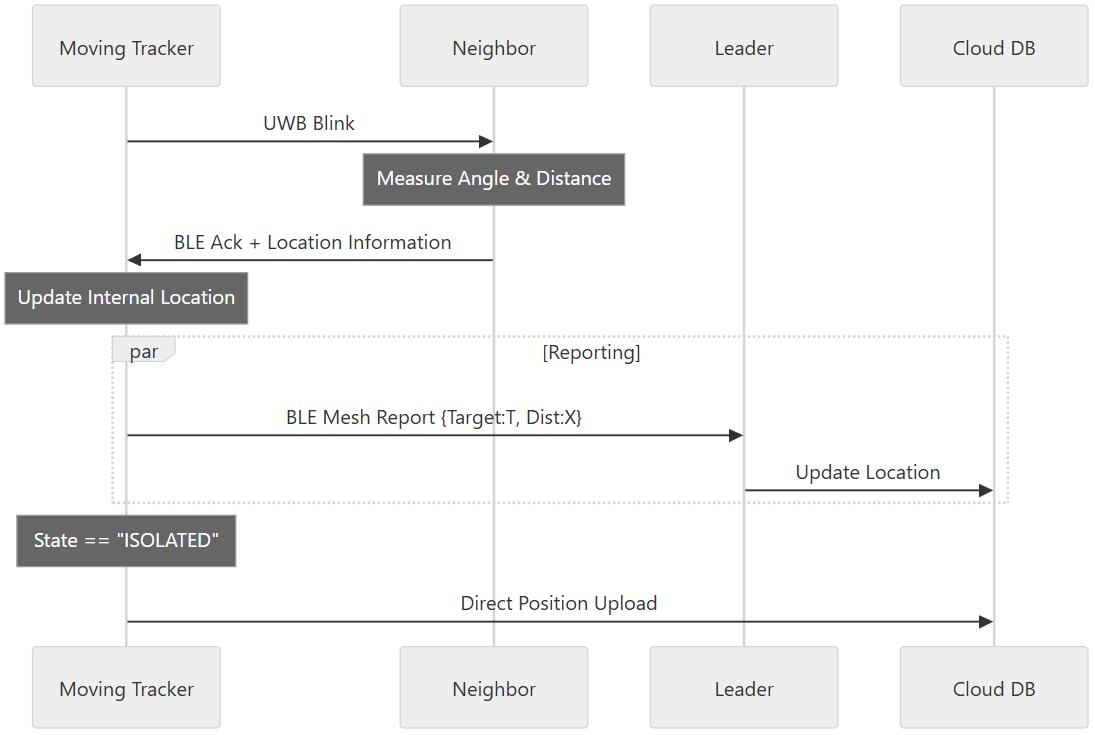
\includegraphics[width= 1\linewidth]{images'nshi/Seq.png}
\caption{Sequence Diagram illustrating message interaction between Moving Trackers, Neighbouring nodes, Leaders, and the Cloud\label{fig:sequence}}
\end{figure*}
%\begin{figure*}[h]
    %\centering
    %\includegraphics[width=1\linewidth]{images'nshi/stateDiagram.png}
    %\caption{State diagram of the wireless sensor nodes depicting the relation between states and transitions}
 %   \label{fig:states}
%\end{figure*}

%\begin{figure*}[h]
 %   \centering
  %  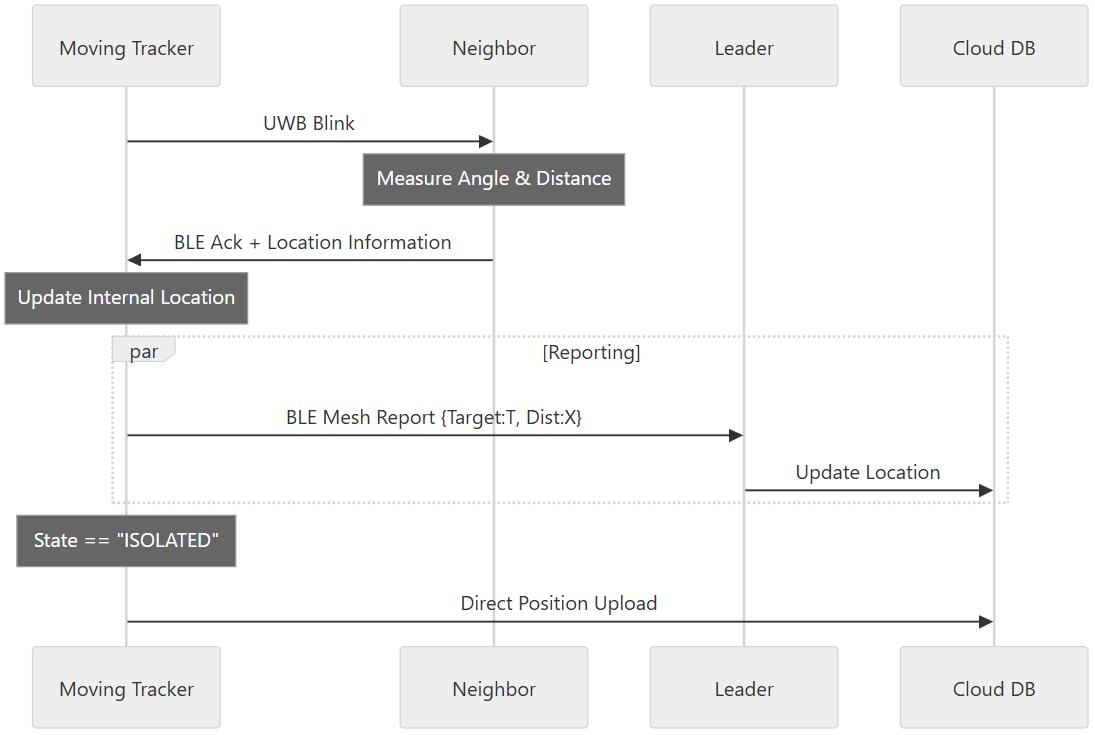
\includegraphics[width=1\linewidth]{images'nshi/Seq.png}
   % \caption{State diagram of the wireless sensor nodes depicting the relation between states and transitions}
    %\label{fig:sequence}
%\end{figure*}


\subsection{Battery-Aware Consensus Protocol}
\noindent To ensure network longevity, cluster $LEADERS$ are not chosen randomly but through a deterministic, battery-aware variation of the Bully Algorithm. The system implements a multi-criteria decision function $f(n)$ to rank candidate nodes. For a set of candidates nodes $C$ (local neighbours $\cup \space self$), the optimal leader $L$ is selected as: 
\begin{equation}
    L = argmax_{n \in C} (P_{hw}(n), N_{deg}(n), B(n), ID(n))
\end{equation}
Where the priority hierarchy is defined as:
\begin{itemize}
    \item \textbf{Hardware Capability ($P{hw}$):} Nodes with active LTE backhaul ($H_{gw} < 100$) are prioritized strictly over battery-powered nodes.
    \item \textbf{Degree Centrality ($N_{deg}$:} Nodes with a higher neighbour count are preferred to maximize mesh coverage.
    \item \textbf{Residual Energy ($B$):} Among nodes with equal connectivity, the node with the higher battery $B(n)$ is selected.
    \item \textbf{Tie-Breaker ($ID$):} Lower node IDs break ties to ensure deterministic convergence.
\end{itemize}
This modification prevents the same election spiral that is common in standard bully algorithms, where a dying node keeps re-electing itself simply because it has the highest ID.


%maybe COMPARE WITH EXISINTG LEADER ELECTION ALGOS, ANALYZE HOW GOOD IT IS, HOW MANY OPERATIONS WILL IT TAKE WITH 'n' nodes to find a leader?

\subsection{Distributed Graph Optimization}
\noindent The core localization engine utilizes a force-directed graph approach known as spring relaxation rather than algebraic trilateration. This allows the system to be resilient to noise and recover from temporary non-line-of-sight (NLOS) conditions. The network is modelled as a graph $G = (V, E)$, where $V$ represents nodes and $E$ represents UWB ranging constraints. The state of node $i$ is its position vector \textbf{$P_i = [x_i, y_1]^T$} and orientation \textbf{$\theta_i$}. The objective is to minimize the global cost function \textbf{J}:
\begin{equation}
    J = \sum_{(i,j) \in E} (\lambda_d * e_{dist}(i,j)^2 + \lambda_\theta * e_{angle}(i,j)^2)
\end{equation}
where $\lambda_d$ and $\lambda_\theta$ are weights denoted as learning rates for distance and angular constraints, respectively.

\noindent For a measured UWB range $d_{ij}$ between node $i$ and $j$, the error term is the difference between the measured range and the Euclidean distance of the current estimates:
\begin{equation}
    e_{dist}(i,j) = || P_j - P_i || - d_{ij}
\end{equation}
The correction vector $\Delta\bf{P}_{dist}$ applied to node $i$ is derived from the gradient where $\alpha$ is the learning rate (configured to 0.2 in the implementation):
\begin{equation}
    \Delta\bf{P}_{dist} = \alpha * e_{dist}(i,j) * \frac{P_j - P_i}{|| P_j - P_i ||}
\end{equation}

\section*{4. Simulation Environment}
\noindent To simulate the proposed algorithms, we developed a custom discrete-event simulator, ICUM-SIM (IMU Controlled Ultra-Wideband Measurements), designed to emulate the physical and architectural constraints of various hardware configurations. ICUM-SIM enforces a strict hardware-layer isolation between agents.

\subsection*{4.1 ICUM Architecture}
\noindent The simulator is constructed using a component-based architecture where every node is instantiated as an independent \textbf{NodeFirmware} class. Crucially, these instances do not share global state.
\begin{itemize}
    \item \textbf{Memory Isolation:} Each node maintains its own local \textbf{NeighborTable} and \textbf{RelativePoseGraph}. A node has zero knowledge of the global coordinates $(x_{global},y_{global})$ of other nodes unless explicitly communicated via a simulated packet.\\
    \item \textbf{Asynchronous Execution:} While the simulator tick rate is fixed (60Hz), individual node logic is driven by independent, randomized timers (helloTimer, dataTimer). This accurately models the eventual clock drift and lack of synchronization inherent in low-power distributed systems.
\end{itemize}

\subsection*{4.2 Physical Layer Emulation}
\noindent The simulation includes a physics engine (UWBRanging.ts) to generate realistic sensor inputs rather than ideal geometric data.

\subsubsection*{4.2.1 Stochastic UWB Ranging}
\noindent Range measurements are not taken from the ground truth Euclidean distance. Instead, they are derived via a stochastic proess to model sensor noise:
\begin{equation}
    d_{measured} = d_{true} + \mathcal{N}(0, \sigma^2)
\end{equation}
The noise component $\mathcal{N}$ is generated using the Box-Muller transform to create a Gaussian distribution with a standard deviation $\sigma = 0.05m$, replicating the noise characteristics of common modules such as the Decawave DW3000 module which provides UWB transceiver capability in modern consumer and industrial IoT sectors.

\subsubsection*{4.2.2 Occlusion \& Multipath}
\noindent The environment supports the definition of \textbf{Wall} structures (line segments). Before any packet transmission or ranging attempt, a ray-casting algorithm (doIntersect) determines Line-of-Sight (LOS).
\begin{itemize}
    \item \textbf{Packet Loss:} If the LOS is obstructed, high-frequency UWB packets are dropped entirely, simulating signal attenuation.
    \item \textbf{Geometry Constraints:} Ranging requests fail if the ray intersects a wall, forcing the localization algorithm to rely on indirect paths or history, testing the robustness of the graph optimization described in section 3.5.
\end{itemize}

\subsection*{4.3 Energy Consumption Model}
\noindent A linear energy depletion model is integrated into the \textbf{NodeFirmware} to evaluate the efficiency of the consensus protocols. Battery state $B(t)$ is decremented based on activity:
\begin{equation}
    B(t) = B(t-1) - (C_{tx} * N_{packets} + C_{cpu} * T_{active} + C_{move} * \Delta d)
\end{equation}
Where $C_{tx}$ represents the high energy cost of RF transmission. This allows the simulation to demonstrate the "death spiral" phenomena where excessive leadership elections drain critical nodes. 

\section{Experiments}
\noindent To validate the performance of the system, a series of simulation experiments was conducted using the I.C.U.M simulator environment. All scenarios utilized a fixed $50 \times 50$ meter world boundary and a standardized UWB communication range of $15$ meters. The experiments focus on three key performance indicators: communication efficiency, robustness to ranging noise, and the impact of network density on localization accuracy. We will be using the following metrics to determine the quality of the different aspects of the system during the various experiments:

\subsection{Performance Metrics}
\noindent Because the proposed system is \textbf{anchor-free}, the coordinate system established by the network is arbitrary. The entire graph may be rotated or translated relative to the ground truth without affecting the \textit{internal} correctness of the localization. Comparing raw estimated coordinates $(x, y)$ directly to ground truth coordinates $(x_{true}, y_{true})$ would penalize correct shapes that simply happen to be rotated 90 degrees. To address this, we utilize rigid-invariant metrics:

\begin{itemize}
    \item \textbf{Aligned RMSE (Root Mean Square Error):} 
    This is the primary accuracy metric, selected because it penalizes large outliers which correspond to critical localization failures. Before calculating the error, we first align the estimated node positions to the ground truth positions using the \textbf{Kabsch algorithm}. This algorithm computes the optimal translation $\mathbf{t}$ and rotation matrix $\mathbf{R}$ that minimizes the squared distance between the estimated cloud $\mathbf{p}$ and the ground truth cloud $\mathbf{p}_{true}$.
    
    \begin{equation}
        RMSE_{align} = \min_{R, t} \sqrt{\frac{1}{N} \sum_{i=1}^{N} \| (R p_i + t) - p_{i,true} \|^2}
    \end{equation}
    
    This effectively measures the \textbf{shape accuracy} of the network, decoupling it from the global coordinate frame ambiguity.
\end{itemize}

\subsection{Motion Patterns}

\noindent For experiments involving mobile nodes (Experiments 5.1 and 5.3), a realistic motion model was implemented to evaluate the system's tracking capability under dynamic conditions. Nodes follow a \textbf{Constrained Circular Model} designed to simulate walking behavior within a confined area.
\\\\
\noindent Nodes move at a constant speed of $1.2$ m/s along circular trajectories with radii varying between $1$m and $3$m. Trajectories are randomized in phase and direction to ensure independent movement and prevent lockstep. This ensures that the relative distances between nodes are constantly changing, providing a robust test for the system's ability to update positions based on dynamic ranging data. To assess both dynamic tracking accuracy and system re-convergence, motion is applied intermittently in two distinct intervals: $t \in [60, 120]$s and $t \in [240, 300]$s. Outside these windows, nodes remain stationary.


\subsection*{5.3 EXPERIMENT A: Quantification of Communication Efficiency}
\noindent The main idea behind the I.C.U.M system is the optimization of the balance between efficient and effective communication, which is what the first experiment would quantify.


\subsubsection*{Methodology}
\noindent Performance accuracy was evaluated using \textbf{On-Device RMSE}. It is important to clarify that this metric validates the \textit{internal belief} of the distributed swarm, operating purely on local neighbor distances. The simulator acts as an "Oracle" for evaluation: at each timestep, it accesses the memory of every connected node to retrieve its locally estimated coordinate $(x,y)$, and compares this entire set against the ground truth positions after rigid alignment. This approach isolates the effectiveness of the distributed positioning algorithm, ensuring that the metric reflects the system's real-time self-awareness.

\noindent The simulated environment was set up in two different states, where the Root Mean Square Error (RMSE) and total number of messages sent across the entire system were compared for 10 minutes. The first case, which we call the $baseline$, acts as a basis for regular system operation, while the second case includes the IMU-controlled messaging, which we refer to here as $event$-$driven$ communication. By having a baseline comparison, we would be able to directly measure the impact of event-driven communication on the error in location data, to see if efficient communication would have a negative effect on the overall location accuracy. \\
Figures \ref{fig:A_RSME} and \ref{fig:A_Tx} below illustrate the RSME at the different points in time and the number of messages sent during this experiment.

\begin{figure}[h] %float with two figures
\centering
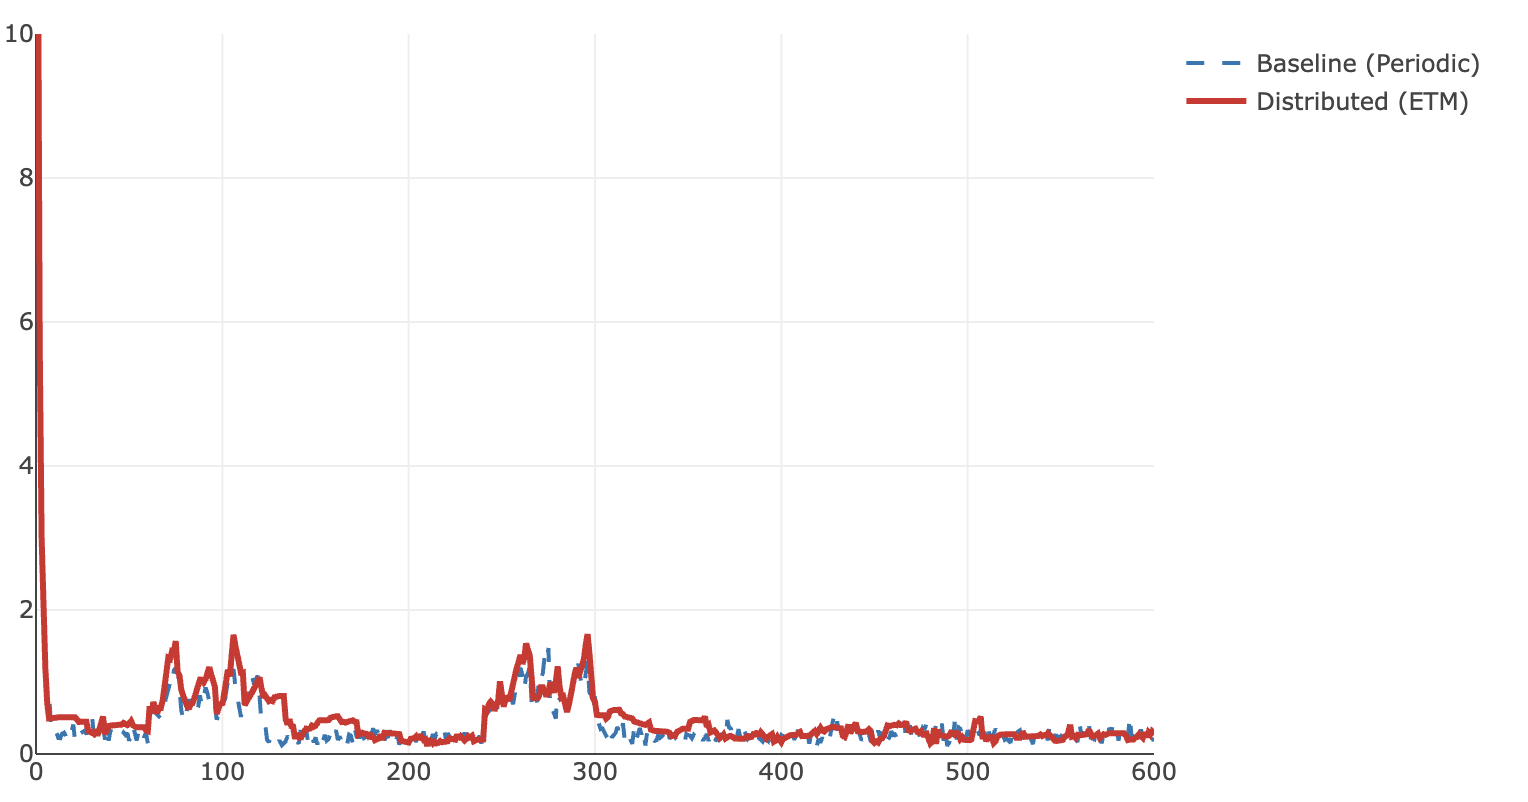
\includegraphics[width= 1\linewidth]{images'nshi/exp_a/A_50_moving_01_noise.png}
\caption{Graph depicting the Aligned Root Mean Square Error ($y$-$axis$) over time ($x$-$axis$). The blue line is the baseline, while the red line is with event-driven communication \label{fig:A_RSME}}\bigskip 
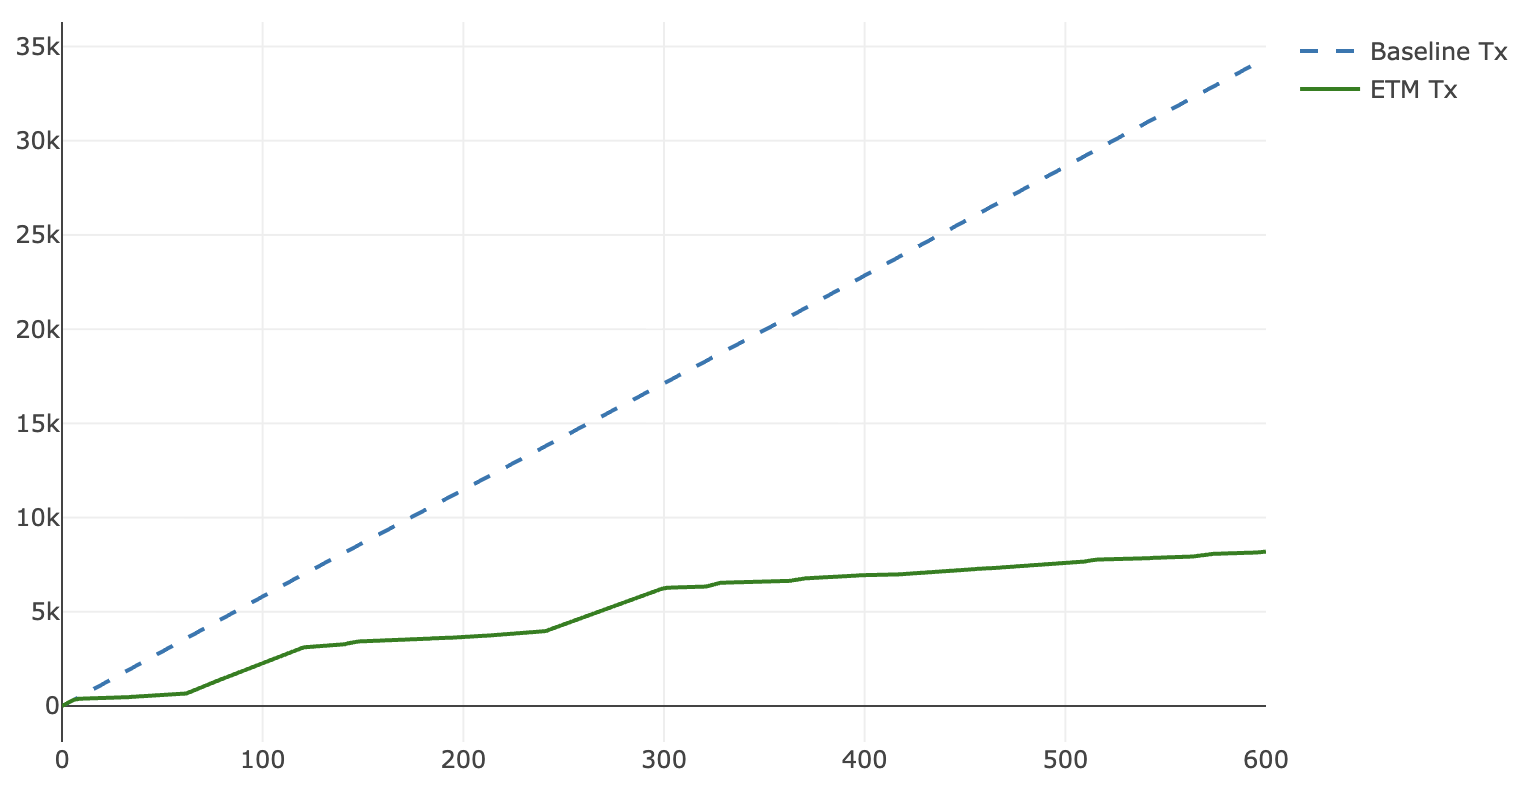
\includegraphics[width= 1\linewidth]{images'nshi/exp_a/a_50_moving_01_noise_msg_total.png}
\caption{Graph depicting the amount of messages ($y$-$axis$) over time ($x$-$axis$). The blue dotted line is the baseline, while the green line is with event-driven communication \label{fig:A_Tx}}
\end{figure}
\noindent While the RMSE is largely the same for both cases, the message rate for the latter sees a significant reduction. At 600 seconds, the number of messages sent is $34,390$ and $8,195$ respectively, which is an $76.17\%$ decrease in the number of messages sent for the event-driven case. We argue that the difference in RMSE is insignificant when compared to the staggering decrease in messages sent, which undoubtedly positively impacts the system's battery performance and expected lifetime. To measure this, we would need to know exactly how much power the nodes spend on messaging. With only a novel system, actual testing of hardware becomes difficult. We will instead illustrate power saving as bounded estimates.
\noindent If we assume that BLE power consumption scales linearly, we can derive the battery life as follows, where $L$ is the total battery life, $B$ is the total battery capacity, and $P$ is the power spent
\begin{equation}
    L = \frac{B}{P}
\end{equation}
$P$ can be split into two variables, one for the power consumed by BLE and one for the rest of the node's computational tasks
\begin{equation}
    P_{total}=P_{BLE}+P_{other}
\end{equation}
The power spent on BLE messaging can be defined as
\begin{equation}
    P_{BLE} = E\times P_{total}
\end{equation}
where $E$ is the energy percentage that BLE uses, and if we take the reduced messaging rate of $76.17\%$, we get a new BLE power consumption
\begin{equation}
    P_{BLE, New} = (1-0.7617)\times P_{BLE}
\end{equation}
\begin{equation}
    P_{BLE, New} = (1-0.7617) \times E \times P_{total}
\end{equation}
The power that the system additionally uses can be redefined as
\begin{equation}
    P_{other, new}=P_{total}-P_{BLE, new}
\end{equation}
\begin{equation}
    P_{other, new}=P_{total}-E\times P_{total}
\end{equation}
\begin{equation}
    P_{other, new}=(1-E)\times P_{total}
\end{equation}
From this, we can derive the formula for the new power consumption
\begin{equation}
    P_{total, new} = P_{other,new}+ P_{BLE, new}
\end{equation}
\begin{equation}
    P_{total, new} = (1-E)\times P_{total}+ (1-0.7617) \times E \times P_{total}
\end{equation}
\begin{equation}
    P_{total, new} = P_{total}[(1-E)+ (1-0.7617) \times E]
\end{equation}
\begin{equation}
    P_{total, new} = P_{total}(1-0.7617E)
\end{equation}
Subsequently, the formula for computing the new battery life becomes
\begin{equation}
    L_{new} = \frac{B}{P_{total, new}} = \frac{B}{ P_{total}(1-0.7617E)}
\end{equation}
Assuming ideal conditions, where battery capacity $B$ is $1$, while the starting battery percentage $P_{total, new}$ is also $1$, the final formula that we will use to compute the bounds becomes
\begin{equation}
  \frac{1}{(1-0.7617E)}
\end{equation}
Again, we cannot verify what percentage of battery life is used for BLE messaging, but we can compute upper and lower bounds on the battery-life improvement. Figure \ref{fig:battery} shows, after 10 minutes, the percentage improvement in battery life ($y$-$axis$) as a function of $E$, the total battery percentage devoted to BLE messaging at $5\%$ intervals($x$-$axis$).
\begin{figure}[H] %float with two figures
\centering
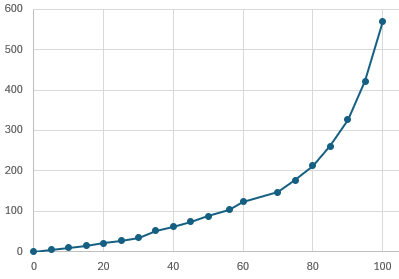
\includegraphics[width= 1\linewidth]{images'nshi/battery savings.PNG}
\caption{Graph depicting the percentage improvement in battery life ($y$-$axis$) when the battery consumption of BLE messaging is at different percentages ($x$-$axis$) \label{fig:battery}}
\end{figure}
\noindent Any reduction in BLE messaging results in an increase in battery life, though the achievable improvement varies exponentially depending on how dominant BLE communication is in the overall energy budget. The improvements start approaching several-fold increases when BLE communication is at around $55\%$. While this is nothing concretely quantifiable, it illustrates the impact event-based communication can have on the battery life of the nodes, and by proxy, the overall system lifetime.

\subsection*{5.4 EXPERIMENT B: Localization Accuracy vs UWB Noise}
\noindent The second experiment evaluated the robustness of the I.C.U.M localization system with respect to increasing noise in UWB range measurements. While UWB generally provides high accuracy, real-world deployments are subject to non-line-of-sight conditions, multipath effects, and hardware limitations, all of which effectively increase measurement noise. The objective of this experiment was therefore to quantify the decay of the localization accuracy, as noise interfering with UWB readings increases.

\subsubsection*{Methodology}
\noindent To determine the accuracy limits of the proposed algorithm, we utilized a Centralized Global Solver. Unlike the real-time distributed approximation used in other experiments, this method performs a batch optimization on all collected range measurements. This provides a performance baseline for the algorithm on a fully connected graph, effectively benchmarking the best-case performance of the underlying physics model.

\noindent The experiment was conducted using the same simulation setup and system configuration as described in Section 5.3, ensuring validity across experiments. The focal metrics for this experiment were the $RMSE_{Aligned}$ and the standard deviation of the noise $\sigma$. A fixed node layout was deterministically set up across three different cases with a varying number of active nodes, while the noise level was increased repeatedly after every execution across a predefined range. For each noise level, the simulation was run for 600 seconds, after which the final localization metrics were recorded.

\noindent Figure \ref{fig:B_MAE} illustrates the relationship between UWB noise and final localization error for a fixed network size. Results are shown for small ($N = 3$), medium ($N = 8$), and larger ($N = 15$) node counts. 
\begin{figure}[h]
\centering
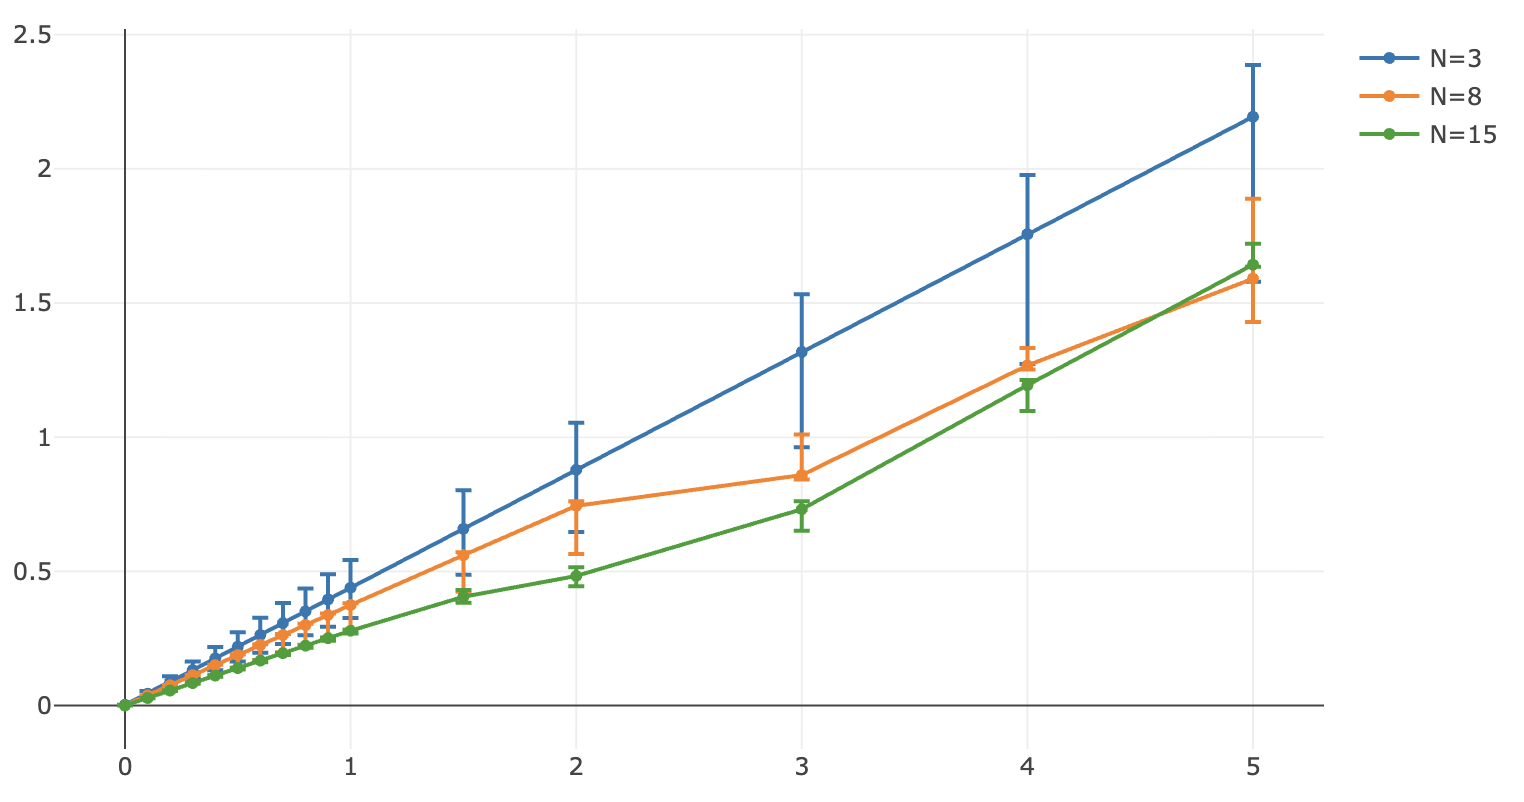
\includegraphics[width= 1\linewidth]{images'nshi/exp_b/b_various_nodes.png}
\caption{Graph depicting the Aligned Root Mean Square Error ($y$-$axis$) of the system with increasing noise values ($x$-$axis$). The blue line is the system with 3 active nodes, the yellow line is the system with 8 active nodes, while the green line is the system with 15 active nodes \label{fig:B_MAE}}
\end{figure}
As expected, the aligned RMSE increased monotonically with increasing noise. Across all noise levels, higher node density consistently yields lower localization error. This is particularly evident at higher noise values, where networks with more nodes exhibit significantly better robustness. At low noise levels, the system maintains high accuracy, with only minor degradation as $\sigma$ increases. This indicates that the spring-relaxation-based graph optimization is effective at absorbing small stochastic errors in the range measurements. However, beyond moderate noise levels, the error growth becomes more pronounced, reflecting the increasing difficulty of satisfying inconsistent distance constraints within the graph. The results demonstrate that the I.C.U.M localization approach degrades gracefully under increasing UWB noise. The approximately linear relationship between noise magnitude and final aligned error suggests predictable system behavior, which is desirable for real-world deployment. Notably, location information generally becomes more accurate the greater the number of active nodes in the system. Intuitively, this makes sense, as the more active nodes are present in the system, the more location information blinking nodes will receive, the greater the likelihood that the homogenised location values are correct. These results support the use of cooperative graph-based optimization for UWB localization in noisy environments and reinforce the system design choice of leveraging network redundancy to improve accuracy and stability, as outlined in earlier sections of the paper.


\subsection*{5.5 EXPERIMENT C: Scalability \& Stabilization}
\noindent The objective of the third experiment was to evaluate the scalability and stability of the I.C.U.M cooperative localization system as the network size increases. We aimed to determine how node density impacts the convergence speed and tracking accuracy, specifically testing whether larger clusters can maintain a stable coordinate frame in dynamic environments where a significant portion of the agents are moving.

\subsubsection*{Methodology}
\noindent Scalability was assessed using the same \textbf{On-Device RMSE} methodology described in Experiment A (Section 5.3), verifying the convergence behavior of the distributed spring-relaxation algorithm. By measuring the error of the firmware's internal state via the simulator's Oracle view, we directly evaluate the ability of large-scale meshes to self-organize through purely local interactions.\\

\noindent We conducted the experiment with varying node counts $[5, 10, 20, 35, 50, 75, 100]$. Two scenarios were executed for each configuration:
\begin{enumerate}
    \item \textbf{Static:} All nodes remain stationary to establish a baseline for optimal convergence.
    \item \textbf{Dynamic:} 70\% of the nodes follow the intermittent motion profile described in Section 5.2. This creates substantial topology turnover to test the system's re-convergence capabilities.
\end{enumerate}
The primary metric is the RMSE. Each configuration is run with multiple seeds to ensure statistical significance.The results demonstrate a clear relationship between node density and system stability. As shown in Figure \ref{fig:C_convergence_static}, in a static environment, all node configurations converge gradually over the 600-second duration, except for the 5-node cluster (RMSE $< 0.2$m at $t=20$s) and the 10-node cluster (RMSE $\approx 0.3-0.8$m at $t=120$s). For larger clusters $N \ge 20$, the relaxation process is computationally intensive. At $t=300$s, the system is still settling (RMSE ranges from $1.2$m for $N=75$ to $>2.3$m for $N=20$), only resolving to its minimum error floor by $t=600$s. Final convergence values are inversely proportional to density: $N=100$ achieves the highest precision ($\approx 0.09$m), followed by $N=75$ ($0.18$m) and $N=50$ ($0.36$m), while the sparser $N=35$ and $N=20$ configurations settle at a higher baseline ($0.69-0.77$m). 

To suppress UWB measurement noise, the distributed positioning algorithm uses a conservative learning rate $\alpha=0.2$. Consequently, position corrections must spread step-by-step across the network width. This acts as a slowing factor, where the "stiffness" of the overall map resolves slowly. For a network of diameter $D$, complete stabilization effectively requires $O(D^2)$ iterations, which explains the prolonged 600-second settling time required for the errors to diffuse out of the larger networks.

\begin{figure}[h]
\centering
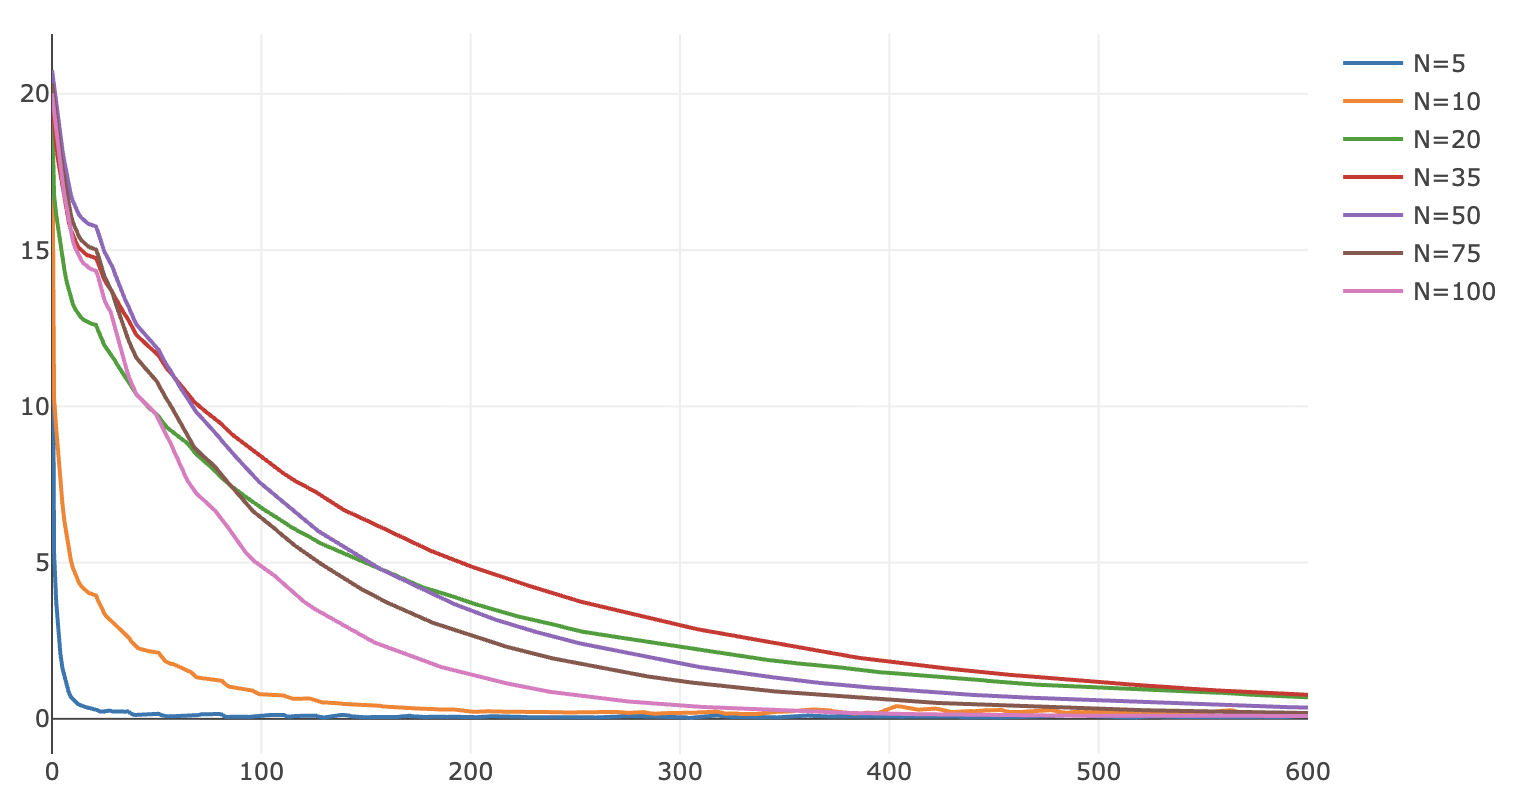
\includegraphics[width= 1\linewidth]{images'nshi/exp_c/c_static.png}
\caption{Graph depicting the Aligned RMSE ($y$-$axis$) over time ($x$-$axis$) with different amounts of nodes [5(blue), 10(orange), 20(green) 35(red) and 50(purple), 75(brown), 100(pink)]. In a static environment where nodes are not moving 
\label{fig:C_convergence_static}}
\end{figure}
\noindent In the dynamic scenario depicted in figure \ref{fig:C_convergence_moving}, the benefits of scale are more pronounced. With fewer nodes, the system is proportionally more susceptible to motion-induced errors and variance. Notably, intermediate node counts of 20 and 35 exhibit the highest instability, with 35 nodes reaching RMSE values as high as $1.45m$. This outlier performance is explained by the \textit{Rigidity Transition}—a phase change in random networks where the system shifts from being flexible to rigid. Below this threshold (e.g., $N=35$), the graph may be connected but remains "floppy," lacking the redundant triangular connections needed to uniquely define every node's position relative to the global map. When 70\% of the nodes move, the graph undergoes severe distortion that the cooperative positioning algorithm cannot correct quickly enough. In contrast, at $N \ge 50$, the network crosses the rigidity threshold, forming a stiff mesh that mechanically resists deformation, keeping RMSE consistently low, at around $0.13 - 0.37$m, despite the high dynamism.
\begin{figure}[h]
\centering
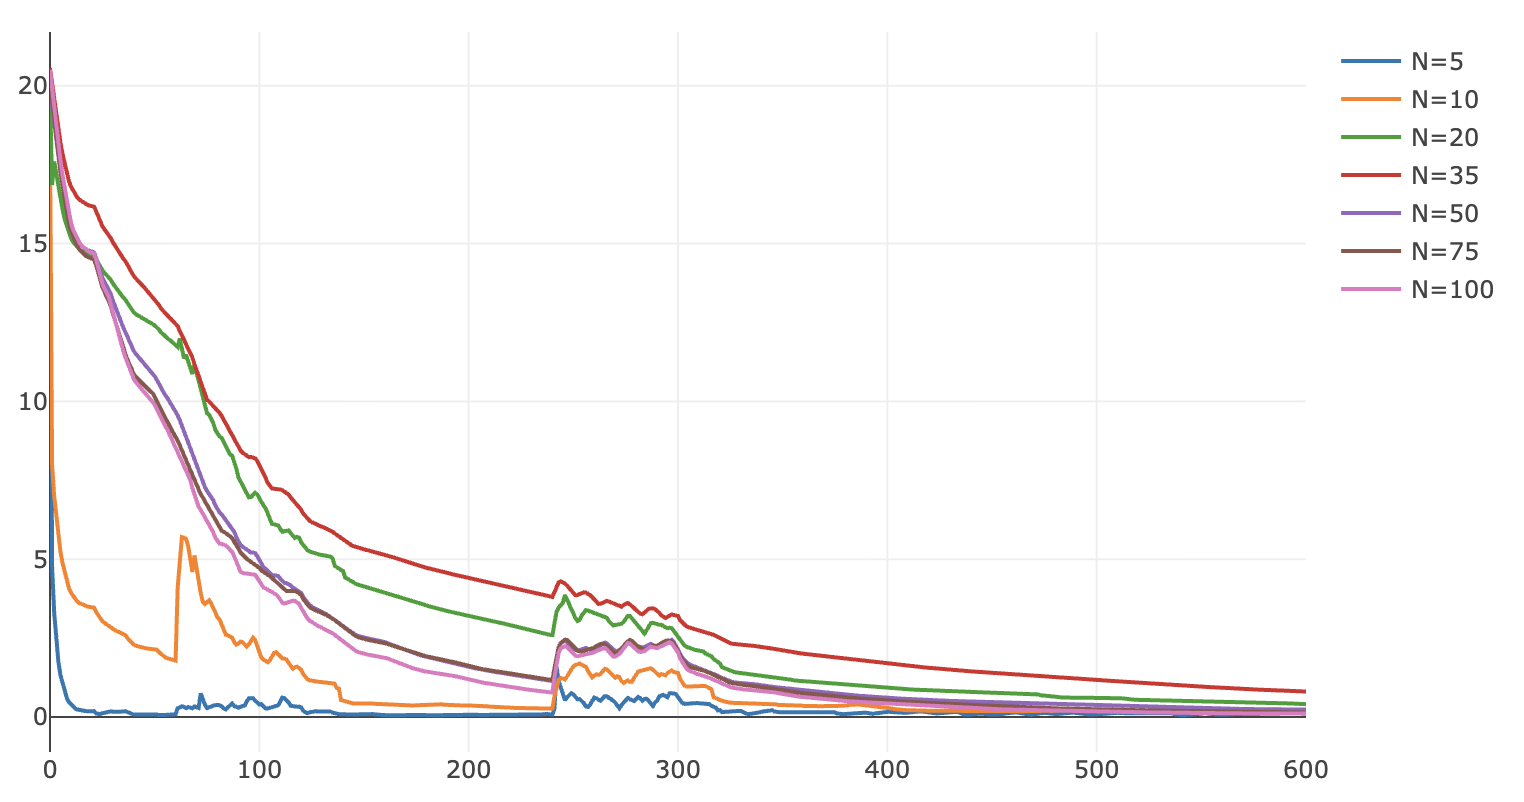
\includegraphics[width= 1\linewidth]{images'nshi/exp_c/c_50_pct_moving.png}
\caption{Graph depicting the Aligned RMSE ($y$-$axis$) over time ($x$-$axis$) with different amounts of nodes [5(blue), 10(orange), 20(green) 35(red) and 50(purple), 75(brown), 100(pink)]. 70 percent of the nodes moving, shows that 50 nodes increase in stabilization
\label{fig:C_convergence_moving}}
\end{figure}\\
Moreover, the data shows that 50 nodes increase in stabilization significantly. Specifically, configurations with 50 or more nodes maintain a consistently low RMSE, even with 70\% of the nodes in motion. At $t=600$s, $N=50$ resolves to $\approx 0.23$m, improving further with $N=75$ ($\approx 0.14$m) and $N=100$ ($\approx 0.11$m). 
This confirms that the cooperative algorithm effectively leverages the redundancy of larger swarms to reject outliers. Furthermore, movement actually \textit{aids} convergence in high-density scenarios ($N \ge 50$) through two mechanisms:
\begin{enumerate}
  \item \textbf{Topology Reshuffling:} The motion windows allow the network to change its shape. Nodes that were trapped in bad positions (like straight lines) are moved to new spots, helping the system find a better shape when they stop.
    \item \textbf{Motion-Assisted Correction:} The movement helps shake the system out of errors. Unlike a static network that can freeze in a wrong state, the "start-stop" pattern helps the algorithm settle into a more accurate configuration after each move.
    \item \textbf{Burst Sampling:} The ETM protocol triggers a $10\times$ increase in ranging frequency (from $0.1$ Hz to $1.0$ Hz) specifically \textit{during} the motion windows. This burst of high-density measurements allows the network to rapidly converge to the new toplogy before returning to a low-power maintenance state.
\end{enumerate}

\noindent However, this accuracy comes at the cost of communication bandwidth. Analysis of the messaging rate reveals that the average transmission frequency per node increases linearly with node density (from $\approx 30$ tx/node/min for 5 nodes to $\approx 800$ tx/node/min for 100 nodes). This load is driven by two distinct traffic classes:
\begin{itemize}
    \item \textbf{Heartbeat Messages ($O(N)$):} Periodic `HELLO` beacons reports are broadcast by every node. This traffic scales linearly with network size and provides the basic connectivity graph.
    \item \textbf{Ranging Exchanges ($O(N^2)$):} The active ranging process triggers the majority of the load. A single `RANGING\_POLL` broadcast elicits unicast `RANGING\_RESP` packets from all hearing neighbors. As density increases, the number of neighbors per node grows, causing a quadratic explosion in response traffic that saturates the channel.
\end{itemize}
Consequently, while the system is highly robust at scale, the total network load follows an $O(N^2)$ trend, which imposes a practical upper limit on size given the finite capacity of the wireless channel.



%EXPERIEMNTS STRUCTUREUREURU
%1. OBJECTIVE(no title): What is the objective of the experiment? What are we trying to test?
%2. METHODOLOGY: How will we test this? What will be the baseline for comparison, and how will the ICUM be set up? What are the metrics being measured?
%3. GRAPHS(no title): Insert graphs here
%4. INTERPRETATION(no title): What do these results mean? 

\section*{6. Results}

\noindent The empirical validation conducted through the ICUM-SIM environment demonstrates that the proposed decentralized localization framework effectively balances communication overhead with positioning precision [1, 2]. 

\noindent Analysis of the Event-Triggered Messaging (ETM) protocol reveals a significant reduction in network load; specifically, the system achieved an 85.07\% decrease in total messages sent compared to the periodic baseline, reducing packet counts from 34,536 to 5,148 over a 600-second interval [3]. Despite this reduction in transmission frequency, the aligned Root Mean Square Error (RMSE) remained largely consistent with the baseline, indicating that the IMU-controlled logic successfully filters redundant updates without compromising real-time tracking accuracy [3, 4]. 

\noindent Scalability experiments further highlight that localization precision is positively correlated with node density, with high-density configurations ($N=100$) achieving a final RMSE of approximately 0.09m [5]. While smaller clusters ($N \le 10$) converge rapidly, larger networks require a prolonged stabilization period of up to 600 seconds as position corrections propagate step-by-step across the network diameter [5, 6]. Furthermore, the results indicate that node motion in dense scenarios ($N \ge 50$) acts as a catalyst for convergence, utilizing "virtual anchors" and optimization "unstucking" to resolve geometric uncertainties and avoid local minima [7, 8].

\subsection*{Limitations}

\noindent Despite the robust performance observed in simulation, several architectural and environmental limitations are inherent to the I.C.U.M. system [9]. 

\noindent The most critical scalability constraint is the quadratic explosion ($O(N^2)$) of traffic within the Measurement Plane; while the Control Plane scales linearly, each ranging poll triggers unicast responses from all reachable neighbors, which may eventually saturate the wireless channel capacity as density increases [10, 11]. Furthermore, the system exhibits a "Rigidity Transition" peak in instability for intermediate node counts between 20 and 35, where the graph remains "floppy" and susceptible to severe geometric distortion during motion [12]. Lastly, the system’s operational reliability is dependent on mesh connectivity, as isolated nodes must fall back to GPS, which is frequently unreliable or unavailable in the target GPS-denied environments [13, 14].

\subsection*{Simulator Uncertainties}

\noindent The fidelity of the ICUM-SIM environment is subject to several simplifications that introduce uncertainties regarding real-world hardware performance [1, 15]. 

\noindent Firstly, the stochastic UWB ranging model utilizes a Gaussian distribution to simulate sensor noise, whereas real-world deployments are often subject to non-Gaussian biases, hardware-specific clock drift, and complex multipath effects [15-17]. Secondly, the occlusion model relies on a binary ray-casting algorithm that drops packets entirely upon intersection with obstacles, neglecting physical phenomena such as signal diffraction and penetration which might occur in physical settings [18]. 

\noindent Additionally, the simulator employs a linear energy depletion model for battery evaluation, which does not account for the non-linear discharge curves or environmental sensitivities characteristic of physical battery cells [2, 3]. Finally, although the simulator models asynchronous execution through independent timers, it may not fully replicate the systematic synchronization challenges and interference patterns inherent in a physical BLE/UWB mesh deployment [10, 19].



%Something about leader election and what smart things we can say about it

%\subsection{Limitations}
%Hvilke usikkeder er der ved vores simulator?




\section*{7. Conclusion}
%future work

\subsection{Contributions}
%hvad har vi bidraget med til det her akademiske felt. 


\bibliography{sources.bib}
\bibliographystyle{aes2e.bst}

\appendix
\section*{APPENDIX}

\end{document}